\section{Auswertung}

Im folgenden lassen sich die aufgenommen Messdaten aus den Tabellen ... bis .. auswerten. Dabei wird zunächst die Grenzspannung $U_{g}$ bei den verwendeten Frequenzen des Lichts mittels linearer Regression ermittelt und es ergeben sich
die Größen $h$/$e_{0}$ sowie die materialabhängige Austrittsarbeit.

%\begin{figure}
%    \centering
%    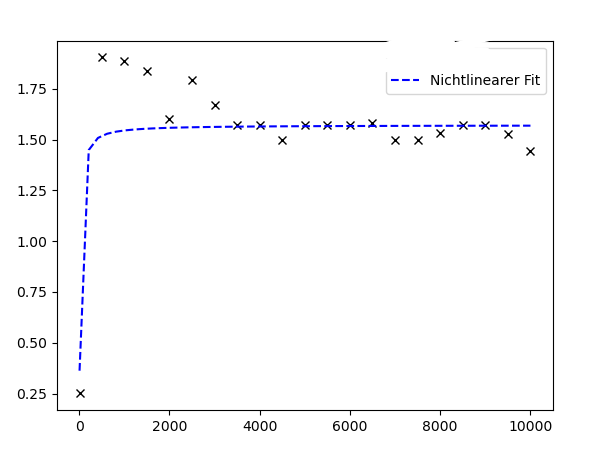
\includegraphics[width=0.5\textwidth]{build/plot1.pdf}
%    \caption{.} 
%    \label{fig:müdes}
%\end{figure}

\subsection{Bestimmung der Grenzspannung}

Zunächst lassen sich für alle aufgenommenen Strom- und Spannungwerte der einzelnen Frequenzen in Abhängigkeit voneinander abbilden. Dabei gilt die Annahme \eqref{eq:whatisthis}, deshalb werden im Folgenden $\sqrt{I}$-$U$ Diagramme dargestellt.
Die Grenzspannungen ergeben sich dabei aus den Spannungwerten bei denen $\sqrt{I} = 0$ gilt.
Für eine genauere Bestimmung der Grenzspannung wird eine lineare Ausgleichsrechnung in der Nähe der Grenzspannung durchgeführt.  Dabei wurden je nach Messreihe unterschiedliche große
Intervalle linearisiert, um genauere Grenzspannungen zu erhalten. 
Die Ausgleichsgeraden wurden hier durch einen \enquote{Polyfit} in Python \cite{python} ermittelt und sind in den jeweiligen Abbildungen ... bis ... mit abgebildet.
\\
Die allgemeine Form der linearen Ausgleichsgeraden sieht folgendermaßen aus
\begin{equation}
    \label{eqn:okay}
y = ax + b.
\end{equation}
Die Parameter $a$ und $b$ sind in den Untertiteln der einzelnen Abbildungen ... bis ... angegeben.

%ABBILDUNGEN

Aus den Schnittpunkten der Ausgleichsgeraden mit der Abszisse ergeben sich die in der Tabelle ... angegebenen Grenzspannungen.


\begin{table}
    \caption{Ermittelte Grenzspannungen $\protect U_{g}$ der einzelnen Messreihen.}
    \centering
    \label{tab:ugrenz}
    \begin{tabular}{c c}
        \toprule
        Wellenlänge $\lambda$ [$\si{\nano\meter}$] & Grenzspannung $U_{g}$ [$\si{\volt}$] \\
        \midrule
        578 & ~\\
        546 & ~\\
        435 & ~\\
        408 & ~\\
        \bottomrule    
    \end{tabular}
\end{table}

\subsection{Bestimmung des Verhältnis von $\protect h$/$\protect e_{0}$}

Zur Bestimmung des Verhältnis der beiden Naturkonstanten $\protect h$/$\protect e_{0}$ werden die zuvor bestimmten Grenzspannungen in Abhängigkeit der verwendeten Frequenz des Lichts $\nu$ dargestellt.
Dieser Zusammenhang wird genau durch Gleichung \eqref{eq:imp} beschrieben. Die Messwerte haben also in der Theorie einen linearen Zusammenhang der sich auch in der Abbildung ... bestätigt.
\\
Wieder kann durch diese Messwerte eine lineare Ausgleichsgerade gelegt werden und die Parameter liefern Aufschluss auf das Verhältnis der Naturkonstanten $\protect h$/$\protect e_{0}$.
Zunächst kann die Gleichung \eqref{eq:imp} nach $U_{g}$ umgeformt werden und es ergibt sich
\begin{equation}
U_{g} = \frac{h}{e_{0}} \nu - \frac{W_A}{e_{0}}
\end{equation}
Ein Koeffizientenvergleich mit der allgemeinen Ausgleichsgeraden \eqref{eqn:okay} liefert die Parameter
\begin{align}
a &= \frac{h}{e_{0}},\\
b &= \frac{W_A}{e_{0}},\\
\end{align}
dabei gibt $a$ die Steigung der Geraden in [$\si{\joule\per\ampere}$] und $b$ die Austrittsarbeit in [$\si{\electronvolt}$] an.